% pre-amble section
\documentclass[11pt,english]{article}
\usepackage[utf8]{inputenc}
\usepackage{geometry}
\usepackage{babel}
\usepackage{hyperref}
\usepackage{graphicx}
\usepackage{appendix}
\usepackage{listings}
\usepackage{caption}
\usepackage{xcolor}

\geometry{legalpaper, margin=1.25in}

\lstdefinestyle{DOS}
{
    backgroundcolor=\color{black},
    basicstyle=\scriptsize\color{white}\ttfamily
}

\title{Herbert\\Autonomous Robotic Rubik's Cube Solver}
\author{
    Jonathan Whitaker\\
    \textt{jon.whitaker@utah.edu}
    \and
    Dylan Lytle\\
    \textt{dylan.lytle@utah.edu}
    \and
    Matt Frandsen\\
    \textt{matt.frandsen@utah.edu}
    \and
    Li Lao\\
    \textt{li.lao@utah.edu}
}
\date{April 2015}
% end of pre-amble

% document content
\begin{document}

\maketitle

\tableofcontents

\section{Abstract}
Project Herbert is an autonomous robotic Rubik's Cube solver that is composed of a complex network of mechanical and electrical devices. In this project our team will be interfacing with these complex mechanical and electrical devices so as to design and create an autonomous robot that is capable of achieving record-breaking Rubik's Cube solution sequences.  This project will be an integration of various technologies including: mechanical actuators, electrical stepper motors, single-board computers, field-programmable gate arrays (FPGAs), and video cameras.

\section{Introduction}
The purpose of this project is to create an autonomous robotic Rubik's Cube solver through the integration of several components. The main components needed in our project include video cameras, electrical stepper motors, mechanical actuators, a single-board computer (SBC), and an FPGA. The video cameras connect to the computer through standard USB 2.0 protocol \cite{USB 2.0}. The video cameras are responsible for capturing the initial configuration of the Rubik's Cube, and the single board computer is responsible for processing the video frame information and generating a matrix model for the initial state of the cube. After generating a matrix model for the initial cube, the computer will then apply Kociemba's algorithm \cite{Kociemba} (an optimal algorithm used to solve a Rubik's Cube) to generate a solution sequence that can be processed sequentially. The solution sequence that Kociemba's algorithm will return will be in the standard notation used in Rubik's Cube discussion and theory (see Appendix \ref{sec:Appendix A}). As each solution sequence is processed, the computer will communicate through an RS232 serial connection to an FPGA board which will drive the mechanical actuation and stepper motor rotations needed to physically manipulate the cube. The FPGA will act as a system control board and will be responsible for controlling the actions of two motor control boards and a relay board used to trigger the mechanical actuators. An overview of this process can be found below in Fig. \ref{fig:System Block Diagram} of section \ref{sec:Project Design}.

Upon completion of the robotic Rubik's Cube solver, if time permits, we hope to take Project Herbert one step further and obtain a Guinness World Record for the fastest robot to solve a Rubik's Cube. CubeStormer3 is the current record holder \cite{GuinnessWR}. The uniqueness of this project is rooted in the optimizations that we will have to make in each component of our system, especially the electro-mechanical stepper motors and the mechanical actuators. We will have to fine-tune these mechanical components to perform physical operations quicker than the human eye in order to obtain record-breaking speed. In this process we will have to maintain the precision needed to rotate the cube.

\section{Project Design}
\label{sec:Project Design}

\begin{figure}[!ht]
\centering
\includegraphics{"Herbert System Diagram".pdf}
\caption{Herbert Block Diagram}
\label{fig:System Block Diagram}
\end{figure}

\subsection{Capturing the Cube with OpenCV}
\label{sec:opencv}

\subsubsection{Camera Orientation}
As seen in Fig. \ref{fig:System Block Diagram}, two cameras will be connected to a SBC through a standard USB 2.0 connection. Each one of these cameras is responsible for capturing exactly three of the six faces of the cube. One camera will capture the front, top, and left faces of the cube. The other camera will be responsible for capturing the back, bottom, and right faces of the cube. To do this, each camera will be positioned so that it faces the corner piece that connects the edges of the faces it is responsible for capturing. An example of this cube orientation is shown in Fig. \ref{fig:Camera Positioning}.

\begin{figure}[!ht]
\centering
\includegraphics[scale=0.25]{"Rubik's Cube Positioning".png}
\caption{Camera Positioning}
\label{fig:Camera Positioning}
\end{figure}

\subsubsection{Utilizing OpenCV for Image Processing}
\label{sec:image processing}
OpenCV is an open source computer vision and machine learning software library \cite{OpenCV}. We will be leveraging this library to perform image analysis on a Rubik's Cube, which will allow us to generate a matrix model for any cube orientation. The OpenCV library will be installed on the SBC, which will enable us to capture and analyze video frames from the USB connected cameras.

Capturing the faces of a cube requires three primary operations:

\begin{enumerate}
  \item \textbf{Grayscale conversion} -
 A video frame will be captured and converted to Grayscale using OpenCV's \textit{cvtColor} function \cite{cvtColor}. Grayscale conversion transforms RGB pixel values into black and white intensity values \cite{Grayscale}. Converting to Grayscale allows an easy transformation to a binary (black and white) image, which is used to filter out features that are not important.
  \item  \textbf{Canny edge detection} -
 Canny edge detection is a multi-stage algorithm used to detect a wide range of edges in an image \cite{Canny Edge Detection}. We will be using OpenCV's \textit{Canny} function \cite{OpenCV Canny} to identify the edges of the Rubik's Cube, which, when combined with contour filtering, will allow us to dynamically identify the planes in the frame that represent the three faces of the cube.

  \item \textbf{Contour filtering} -
 Contour filtering will be used to identify the contours of the Rubik's Cube within the image. OpenCV's \textit{findContours} function \cite{findContours} will allow us to identify the region of space in the image where the Rubik's Cube resides. Likewise, it will enable us to identify individual cubelets on each of the three faces of the cube.
\end{enumerate}

After the individual cubelets have been identified within the image, a matrix model like that shown in Fig. \ref{fig:matrix layout} will be generated. Each individual position (U1, U2, F1, F2, etc.) can be represented as a single ASCII character indicating the color at that cubelet position. Table \ref{table:cubelet representation} defines the mapping scheme we will employ for the Rubik's Cube matrix model. Once this matrix model has been generated for the cube, we will pass it on to an application known as \textit{Kcube}. Kcube will process the cube permutation (see \ref{sec:Kcube}), apply Kociemba's algorithm, and generate a solution sequence.

\begin{figure}[!ht]
\centering
\begin{verbatim}
             |************|
             |*U1**U2**U3*|
             |************|
             |*U4**U5**U6*|
             |************|
             |*U7**U8**U9*|
             |************|
|************|************|************|************|
|*L1**L2**L3*|*F1**F2**F3*|*R1**R2**F3*|*B1**B2**B3*|
|************|************|************|************|
|*L4**L5**L6*|*F4**F5**F6*|*R4**R5**R6*|*B4**B5**B6*|
|************|************|************|************|
|*L7**L8**L9*|*F7**F8**F9*|*R7**R8**R9*|*B7**B8**B9*|
|************|************|************|************|
             |************|
             |*D1**D2**D3*|
             |************|
             |*D4**D5**D6*|
             |************|
             |*D7**D8**D9*|
             |************|
\end{verbatim}
\caption{Rubik's Cube matrix representation}
\label{fig:matrix layout}
\end{figure}

\begin{table}[!ht]
\centering
\begin{tabular}{|c|c|}
\hline
\textbf{COLOR} & \textbf{CHARACTER} \\ \hline
WHITE          & 'W'              \\ \hline
RED            & 'R'              \\ \hline
BLUE           & 'B'              \\ \hline
GREEN          & 'G'              \\ \hline
ORANGE         & 'O'              \\ \hline
YELLOW         & 'Y'              \\ \hline
\end{tabular}
\caption{Cubelet color to ASCII character mapping}
\label{table:cubelet representation}
\end{table}

\subsection{Kcube and the Solution Sequence}
\label{sec:Kcube}
Kcube is a C++ application developed by Greg Schmidt that utilizes Kociemba's two-phase algorithm which uses two stages of an iterative depth first search algorithm \cite{The Two-Phase Algorithm}. The Kcube application will be used to generate the solution sequence needed to solve the Rubik's Cube that was captured during the image processing phase. The matrix model generated from the image processing phase will allow us to provide Kcube's command-line interface with the cube representation needed to generate a solution sequence. Kcube's command-line interface takes six parameters, one for each face of the cube. The values for these parameters are the color characters at each of the cubelet locations for that face (as seen in Fig. \ref{fig:matrix layout}). For example, to solve the scrambled cube shown in Fig. \ref{fig:scrambled cube} you would invoke Kcube with the following command:

\begin{lstlisting}[style=DOS]
Microsoft Windows [Version X.X.XXX]
Copyright (c) 2015 Microsoft Corporation. All rights reserved.

c:>kcube L:GGWWOWBRB F:GWGBGYWBO U:YOOOWYROY D:ORGWYYYRB R:OGBBRYWRR B:YBROBGWGR
\end{lstlisting}

Kcube will then process the input parameters and generate a sequence of twenty-three or less moves (see \ref{sec:fundamental moves}) that, when applied to the cube, will solve the cube. Each move will be mapped to a unique integer value (see Table \ref{table:moves table}), and these values will be transmitted sequentially over an RS232 serial connection to the FPGA control board, at which point the control board will take responsibility for controlling the electro-mechanical stepper motors and mechanical actuators needed to physically manipulate the cube.


\begin{figure}[!ht]
\centering
\includegraphics[scale=1.25]{"Scrambled Cube".jpg}
\caption[]{}
\label{fig:scrambled cube}
\end{figure}

\begin{table}[!ht]
\centering
\begin{tabular}{|c|c|c|c|c|c|}
\hline
\textbf{MOVE} & \textbf{VALUE} & \textbf{MOVE} & \textbf{VALUE} & \textbf{MOVE} & \textbf{VALUE} \\ \hline
F             & 1              & R             & 7              & D             & 13             \\ \hline
F'            & 2              & R'            & 8              & D'            & 14             \\ \hline
F2            & 3              & R2            & 9              & D2            & 15             \\ \hline
L             & 4              & U             & 10             & B             & 16             \\ \hline
L'            & 5              & U'            & 11             & B'            & 17             \\ \hline
L2            & 6              & U2            & 12             & B2            & 18             \\ \hline
\end{tabular}
\caption{Cube moves to integer mapping}
\label{table:moves table}
\end{table}

\subsection{Mechanical Actuators}
\label{sec:Mechanical Actuators}
To physically manipulate the cube, Herbert will employ a six arm design. One arm for each face of the cube. In order to achieve a six arm design, each arm must actuate in and out so as to avoid conflict
with the other arms. This actuation process is a time critical component of
the design, and therefore needs to be as fast as possible.  We initially planned on implementing the
arm actuation with motors.  However, preliminary testing has showed that using
motors to convert rotary motion into linear motion is too slow, and using a linear motor
actuator is too costly. Our design requires high speed and affordable cost. We believe pneumatic actuation is the solution to this problem.  Each of the arms will be attached to a double action pneumatic air cylinder as show in Fig. \ref{fig:Pneumatic Air Cylinder}.

\begin{figure}[!ht]
\centering
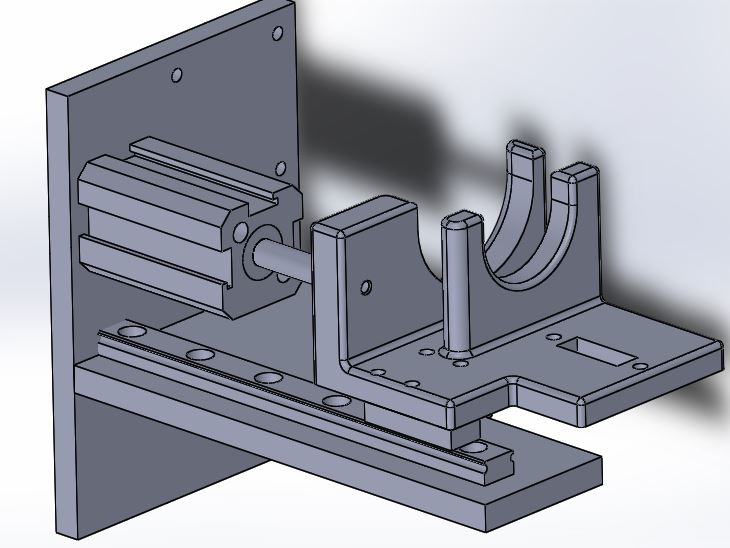
\includegraphics[scale=0.5]{AirCylinder.jpg}
\caption{Pneumatic Air Cylinder}
\label{fig:Pneumatic Air Cylinder}
\end{figure}

The FPGA control board will be responsible for controlling a relay control board (see Fig. \ref{fig:System Block Diagram}) which will control coaxial pairs of air cylinders. The actuation distance for each control arm will be fixed. The relay switches coaxial pairs of arms will either be in an extended or retracted position. Potential optimizations and more stable cube manipulations  are obtained by simultaneously extending and retracting coaxial pairs of arms. The linear actuation motion allows two coaxial pairs of
arms to extend, thus encasing two sides of the cube in the sockets of the arms. After a pair of arms extend,
a stepper motor will spin the arm corresponding to the appropriate move from the solution sequence (see section \ref{sec:Stepper Motors}). Each air cylinder will be provided approximately 80-100 psi supplied from an air compressor. To protect against any
arm collisions only one pair of arms will be in the extended position at any given time.


\subsection{Electro-mechanical Stepper Motors}
\label{sec:Stepper Motors}
Each actuating arm will have a stepper motor which will be responsible for rotating a single face. A stepper motor will rotate a face either 90 degrees or 180 degress clockwise or counter-clockwise based on the solution move that is being processed (as specified in Appendix \ref{sec:Appendix A}). A square axle (as seen Fig. \ref{fig:Stepper Motor Arm}) will be fastened to the stepper motors. This axle will twist the arm pieces in order to spin the faces of the Rubik's Cube.

\begin{figure}[!ht]
\centering
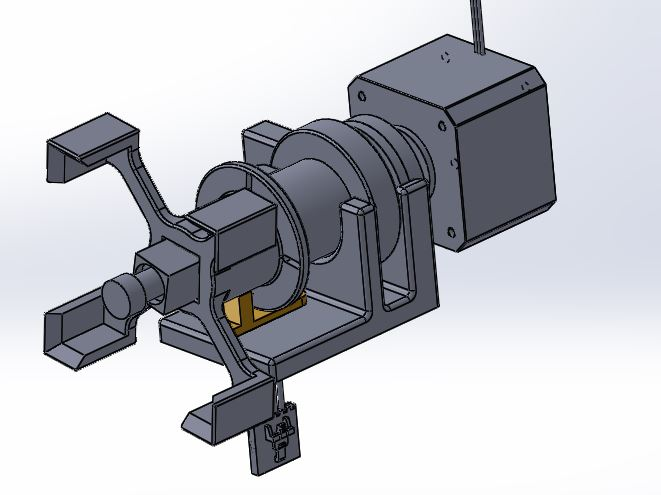
\includegraphics[scale=0.5]{StepperMotorArm.jpg}
\caption{Stepper Motor Arm}
\label{fig:Stepper Motor Arm}
\end{figure}

Each stepper motor will be driven by a motor control board which will be controlled by the FPGA control board (see Fig. \ref{fig:System Block Diagram}). The motor control boards will contain a motor driver chip for each stepper motor. The FPGA control board will be responsible for controlling the angular and temporal timing of each stepper motor rotation.


\section{Schedule}
Our work will be distributed over the upcoming summer months and Fall 2015 semester, spanning May 13-December 2015. Table \ref{table:herbert timeline} outlines the milestones we hope to have completed by the end of this upcoming summer. A brief description of each one of these milestones is presented in Section \ref{sec:Milestones}. Comes Fall semester 2015, we hope to be integrating each component and testing the robustness of our system.
\begin{table}[!ht]
\resizebox{\textwidth}{!}{\begin{tabular}{|l|c|c|c|}
\hline
\multicolumn{1}{|c|}{\textbf{Tasks}}      & \textbf{Start} & \textbf{Finish} & \textbf{Milestone}                 \\ \hline
\textbf{}                                 & 2015-05-13     & 2015-05-20      & OpenCV Setup                       \\ \hline
Setup Windows Embedded VM using Vagrant   &                &                 &                                    \\ \hline
Install Camera Drivers and Interfaces     &                &                 &                                    \\ \hline
Download and Install OpenCV               &                &                 &                                    \\ \hline
\textbf{}                                 & 2015-05-20     & 2015-06-19      & Basic Cube Capture                 \\ \hline
Research Object Detection Algorithms      &                &                 &                                    \\ \hline
Experiment with Canny Edge Detection      &                &                 &                                    \\ \hline
Experiment with Contour Identification    &                &                 &                                    \\ \hline
                                          & 2015-06-19     & 2015-07-02      & Finalize Object Detection Software \\ \hline
Implement Object Detection Algorithm      &                &                 &                                    \\ \hline
Generate Output Representation of Cube    &                &                 &                                    \\ \hline
\textbf{}                                 & 2015-05-13     & 2015-05-26      & Mechanical Tasks                   \\ \hline
Build The Herbert Frame                   &                &                 &                                    \\ \hline
Determine fastener hardware               &                &                 &                                    \\ \hline
Gather Hardware                           &                &                 &                                    \\ \hline
Print 3D Arms                             &                &                 &                                    \\ \hline
Attach Hardware to Frame                  &                &                 &                                    \\ \hline
\textbf{}                                 & 2015-05-13     & 2015-06-12      & Firmware for Solution Sequence     \\ \hline
Implement firmware for solution execution &                &                 &                                    \\ \hline
Create Offline Command in comm.c          &                &                 &                                    \\ \hline
\textbf{}                                 & 2015-06-15     & 2015-07-10      & Herbert Test Application           \\ \hline
Add tab for Basic Movements               &                &                 &                                    \\ \hline
Add tab for Manual Solution Input         &                &                 &                                    \\ \hline
Add tab for testing motors and sensors    &                &                 &                                    \\ \hline
                                          & 2015-12-16     & 2015-07-11      & Integration and Testing            \\ \hline
T.B.D.                                    &                &                 &                                    \\ \hline
\end{tabular}}
\caption{Herbert itemized timeline}
\label{table:herbert timeline}
\end{table}

\subsection{Milestones}
\label{sec:Milestones}
\begin{itemize}
  \item {\bf OpenCV Setup} \hfill \\
  In this milestone we will configure a stable development environment for OpenCV, which will include setting up a development box, installing camera device drivers, and installing and configuring OpenCV.

  \item {\bf Basic Cube Capture} \hfill \\
  In this milestone we will familiarize ourselves with the OpenCV technologies and experiment with Canny edge detection and contour identification algorithms. This will give us the background we need to implement our cube capture application.
  \item {\bf Kcube and the Solution Sequence} \hfill \\
  By the end of this milestone we will be able to capture a cube, process it using the Kcube application, and generate a solution sequence that can be passed on to the FPGA control board for further processing.

  \item {\bf Mechanical Tasks} \hfill \\
  This milestone is dedicated to getting all of the mechanical parts integrated. This includes fastening the electro-mechanical stepper motors to the actuating arms and connecting the arms to the main chassis. Upon completion of this milestone we should have functioning mechanical components and a  working robot skeleton that can be operated by the FPGA control board.

  \item {\bf Firmware for Solution Execution} \hfill \\
  By the end of this milestone all FPGA control board firmware should be finalized and tested. When given a solution from Kcube, Herbert should be able to carry out the operations needed to solve the cube.

  \item {\bf Herbert Test Application} \hfill \\
  This goal of this milestone is to create a test application that allows us to interact with the mechancial components through a software interfaces communicating through the firmware on the FPGA control board. At the end of this milestone we should be able to manually control the rotation and actuation of the mechanical arms.

  \item {\bf Integration and Testing} \hfill \\
  Every part should be integrated together and tested for robustness and speed by the end of this milestone. If there are any errors or optimizations needed, then they are done upon completing this milestone as well. This milestone is tentatively scheduled after every other milestone is completed.
\end{itemize}


We believe that parallelizing these tasks by distributing them across our team will allow us to design this system in a time efficient manner. We hope to stay close to the timeline we present above, however the timeline is tentative, and will likely change over the course of summer and Fall semester.

\section{Required Resources}
Herbert system diagram shown in figure \ref{fig:System Block Diagram}, outlines some of the main system components of project Herbert.
These components are crucial to the design and success of this project. Each component and its main functionality is as follows.
Cameras which are used to acquire the data.
Single board computer to process the data.
FPGA, motor control boards, relay board, and sensors to control the system.
Stepper motors, 3D printed materials, pneumatic air cylinders, and solenoid valves to perform the work.
Below in table \ref{table:main component bom} is a BOM for these items
\begin{table}[!ht]
\begin{tabular}{|c|c|c|c|c|}
\hline
\textbf{Part Description} & \textbf{Quantity} & \textbf{Vendor}     & \textbf{Vendor PN} & \textbf{Price/Unit} \\ \hline
Stepper Motor             & 6                 & BioFire Scrap       & NA                 & 0.00                \\ \hline
Air Cylinder              & 6                 & Amico               & a12030500ux0057    & 7.86                \\ \hline
Solenoid Valve            & 6                 & Uxcell              & a11102700ux0130    & 10.31               \\ \hline
System Control Board      & 1                 & BioFire Scrap       & NA                 & 0.00                \\ \hline
Motor Control Board       & 2                 & BioFire Scrap       & NA                 & 0.00                \\ \hline
Relay Board               & 1                 & SainSmart           & 20-018-102         & 11.99               \\ \hline
Camera                    & 2                 & Point Grey Research & Chameleon 3        & 0.00                \\ \hline
\end{tabular}
\caption{Main Component BOM}
\label{table:main component bom}
\end{table}

\section{Risk Assessment}

The main risk associated with this project is the image processing. The likelihood of error in the cube capture phase is high. Capturing the cube orientation is error-prone because of changes in environmental lighting conditions. Object detection algorithms present a steep learning curve. Likewise, interfacing with camera device parameters to aid in eliminating changes in ambient lighting can further increase the complexity of obtaining the initial cube configuration. Capturing the initial cube state is a core component of this project. Without accurate cube capture, the autonomous aspect of our project is void. As a result of this, we will put a large emphasis on accurate cube capture. If adapting to various lighting conditions proves too difficult and becomes too time costly, we will design our system under ideal lighting conditions to eliminate this risk altogether.

Another high risk component of project Herbert is the chance of mechanical failure. There are various mechanical components that could cause total system failure if they were to break. If mechanical failures occur, the entire project may be jeopardized. In order to mitigate this risk, we have made sure that spare hardware parts can be obtained quickly from our industry sponsors.

\section{Summary}

Project Herbert is a project that integrates various technologies and domains of engineering into one complete package. It will be broken down into three primary parts: cube detection, solution generation, and the physical manipulation of the cube using mechanical components. Each of these
will present their own set of challenges. Implementing the cube detection application will require a lot of research in the field of image processing/computer vision, especially if we attempt to operate the system under various lighting conditions. The mechanical
aspect of this project will require a fundamental understanding of mechatronics and robotics. The mechanical aspect of this proejct will also pose the greatest limitations. We will have to optimize the mechanical components by reducing frictional effects so as to ensure operation timings that are
within the window of time needed to solve a cube in record breaking time.

The workload associated with this project is ambitious. As a result of this, the workload will be distributed and worked on in parallel over the upcoming summer
and Fall 2015 term. Working in parallel over the summer will allow us to get the bulk of the individual components implemented before Fall term, which will allow us to focus on integration, testing, and
optimizations over the Fall semester. Thanks to many industry sponsors we are confident that the risks associated with our project will be mitigated in the case of component failure. This will allow
us to focus the majority of our time on design, integration, and testing.

\section{Acknowledgements}
Our team would like to thank BioFire Defense LLC, Point Grey Research Inc., and Futura Industries for all the support and resources they have provided us. Your contributions are greatly appreciated.


\begin{figure}[!htb]
\minipage{0.32\textwidth}
  
\includegraphics[width=\linewidth]{biofire_logo.png}
  \label{fig:biofire_logo}
\endminipage\hfill
\minipage{0.32\textwidth}
  
\includegraphics[width=\linewidth]{point_grey.png}
  \label{fig:point_grey}
\endminipage\hfill
\minipage{0.32\textwidth}%
  
\includegraphics[width=\linewidth]{futura_indust.jpg}
  \label{fig:futura_indst}
\endminipage
\label{fig:project_sponsors}
\end{figure}

BioFire Defense has given us the various control boards and mechanical components needed for this project. They have also given us access to various prototyping tools including high precision 3D printers and laser cutters. A special thanks goes out to BioFire engineers Logan Taylor (Mechanical), Pat Riley (Electrical/Systems), Matt Murdock (Electrical), and David Nielsen (VP of Product Development). These individuals have provided invaluable time and knowledge to our team.

We'd also like to thank Vladimir Tucakov of Point Grey Research. He has provided our team with their Chameleon CMLN-13S2M-CS camera which we will use for precise and fast image acquisition. Vladimir has also discussed our project and ideas with his colleagues at Point Grey, and they have mentioned featuring our project in their newsletter.

We couldn't put all these components together without a nice chassis to house them all. For this, we would like to thank Futura Industries. They have helped us in the design and construction of the aluminum frame we will use to build Herbert. Another special thanks goes out to Futura's Kenton Frandsen (Mechanical/Manufacturing Engineer) who has assisted in the mechanical design of the arm and frame of our project.

\begin{thebibliography}{9}
\bibliographystyle{IEEEtran}

\bibitem{USB 2.0}
\emph{USB 2.0 Specification}
[Online]. Available: \url{http://www.usb.org/developers/docs/usb20_docs/}

\bibitem{Kociemba}
Herbert Kociemba.
\emph{The Two-Phase Algorithm}
[Online]. Available: \url{http://kociemba.org/cube.htm}

\bibitem{GuinnessWR}
Guinness World Records.
\emph{Fastest robot to solve a Rubik's Cube}
[Online]. Available: \url{http://www.guinnessworldrecords.com/world-records/fastest-robot-to-solve-a-rubiks-cub}

\bibitem{OpenCV}
OpenCV Developers Team.
\emph{About OpenCV}
[Online]. Available: \url{http://opencv.org/about.html}

\bibitem{cvtColor}
OpenCV Developers Team.
\emph{Miscellaneous Image Transformations}
[Online]. Available: \url{http://docs.opencv.org/modules/imgproc/doc/miscellaneous_transformations.html#cvtcolor}

\bibitem{Grayscale}
Wikipedia contributors.
\emph{Grayscale}
[Online]. Available: \url{http://en.wikipedia.org/w/index.php?title=Grayscale&oldid=652694198}

\bibitem{Canny Edge Detection}
Wikipedia contributors.
\emph{Canny edge detector}
[Online]. Available: \url{http://en.wikipedia.org/w/index.php?title=Canny_edge_detector&oldid=655662708}

\bibitem{OpenCV Canny}
OpenCV Developers Team.
\emph{Feature Detection}
[Online]. Available: \url{http://docs.opencv.org/modules/imgproc/doc/feature_detection.html?highlight=canny#canny}

\bibitem{findContours}
OpenCV Developers Team.
\emph{Structural Analysis and Shape Descriptors}
[Online]. Available: \url{http://docs.opencv.org/modules/imgproc/doc/structural_analysis_and_shape_descriptors.html?highlight=findcontours#findcontours}

\bibitem{Basic Cube Notation}
Joseph Converse.
\emph{Basic Notation}
[Online]. Available: \url{http://astro.berkeley.edu/~converse/rubiks.php?id1=basics&id2=notation}

\bibitem{The Two-Phase Algorithm}
Herbert Kociemba
\emph{The Two-Phase Algorithm}
[Online]. Available: \url{http://kociemba.org/twophase.htm}
\end{thebibliography}

\appendix
\section{Rubik's Cube Notation and Terminology}
\label{sec:Appendix A}
In order to solve a cube, it is standard to define the terminology and orientation layout used in Rubik's Cube theory and analysis. This section describes the basic notation that is used throughout this document.

\subsection{Faces}
A Rubik's Cube is composed of six faces: right (\textbf{R}), left (\textbf{L}), up (\textbf{U}), down (\textbf{D}), front (\textbf{F}), and back (\textbf{B}) (see Fig. \ref{fig:Cube Orientation}). The exact color of each face is relative to the orientation in which you are holding the cube. For example, if you align the blue face towards you then the blue face is defined as the front face. Each face can be rotated in two different directions: \textit{clockwise} or \textit{counter-clockwise}. These rotations are defined as the direction of rotation when looking directly at that face.

\begin{figure}[!ht]
\centering
\includegraphics{"Cube Orientation".png}
\caption{Cube orientation}
\label{fig:Cube Orientation}
\end{figure}

\subsection{Fundamental Moves}
\label{sec:fundamental moves}
The most fundamental moves are 90-degree clock-wise rotations for each of the faces outlined above. These moves are outlined below \cite{Basic Cube Notation}:

\begin{itemize}

\item{\textbf{R}} - Indicates a 90-degree clockwise rotation of the right face such that the side on top rotates towards the back.
\item{\textbf{L}} - Indicates a 90-degree clockwise rotation of the left face such that the side on top rotates towards the front.
\item{\textbf{U}} - Indicates a 90-degree clockwise rotation of the upper face such that the side in front moves to the left.
\item{\textbf{D}} - Indicates a 90-degree clockwise rotation of the downward face such that the side in front moves to the right.
\item{\textbf{F}} - Indicates a 90-degree clockwise rotation of the front face such that the side on top moves to the right.
\item{\textbf{B}} - Indicates a 90-degree clockwise rotation of the back face such that the side on top moves to the left.
\end{itemize}

\subsection{Modifiers}
For each of the fundamental moves above, there are modifiers that can be appended to the move to change the rotation of the face. My example below uses \textbf{L} as the base move, but these modifiers can be applied to any of the fundamental moves.

\begin{itemize}
\item \textbf{L'} - Indicates a 90-degree counter-clockwise rotation of the left face such that the side on top rotates towards the back (opposite direction as that defined above).
\item \textbf{L2} - Indicates a 180-degree rotation of the left face (two rotations).
\end{itemize}

\subsection{Cubelets}
A cubelet refers to a particular piece on the cube. Cubelets are categorized based on their position. There are three types of cubelets: center cubelets, edge cubelets, and corner cubelets (see Fig. \ref{fig:cubelet_categories}). A center cubelet is unique. All other cubelets revolve around the center cubelets, they never move (go ahead, try and move the center piece). Edge cubelets connect two face pieces together at an edge. A corner cubelet connects three pieces together at the corner of the cube.

\begin{figure}[!htb]
\minipage{0.32\textwidth}
  \includegraphics[width=\linewidth]{"Center cubelets".png}
  \label{fig:center_cubelets}
\endminipage\hfill
\minipage{0.32\textwidth}
  \includegraphics[width=\linewidth]{"Edge cubelets".png}
  \label{fig:edge_cubelets}
\endminipage\hfill
\minipage{0.32\textwidth}%
  \includegraphics[width=\linewidth]{"Corner cubelets".png}
  \label{fig:corner_cubelets}
\endminipage
\caption{Cubelet categories}
\label{fig:cubelet_categories}
\end{figure}



\end{document}
% end of document content
